\section{介绍Oxford Nanopore的原理、优缺点、应用}


牛津纳米孔技术Oxford Nanopore属于第三代DNA测序技术,其特点是单分子测序、实时测量和较长读长,从而大幅提升测序速度和准确性.英国的牛津纳米孔技术有限公司(Oxford Nanopore Technologies, ONT)专注于开发和销售纳米孔测序产品(如便携式DNA测序仪MinION,2014)\cite{1deamer2016three}\cite{2jain2016oxford},用于单分子的直接、电子分析.

自2014年提供首台纳米孔测序仪MinION以来,纳米孔测序技术及其在基础和应用研究中的应用得到了显著增长.纳米孔技术的快速发展带来了单个长DNA和RNA分子测序准确性、读长和吞吐量的大幅提升.为充分利用纳米孔长读长研究基因组、转录组、表观基因组和表观转录组,需要广泛发展实验和生物信息学方法.纳米孔测序应用于基因组组装、全长转录本检测、碱基修饰检测等领域,以及快速临床诊断和疫情监测等专门领域.通过开发新纳米孔、碱基调用方法和为特定应用定制实验方案,仍有数据质量和分析方法的问题值得改进.

\subsection{Oxford Nanopore牛津纳米孔测序技术的原理}

\subsubsection{Minion技术原理和测序步骤}
具体来说,我们这里主要讨论Oxford Nanopore推出的首款纳米孔测序设备MinION的技术原理.该技术依赖于纳米级蛋白质孔,即“纳米孔”,作为生物传感器,嵌入耐电性聚合物膜中.在电解液中,施加恒定电压产生流过纳米孔的离子电流,从而使带负电荷的单链DNA或RNA分子从带负电荷的顺式侧向带正电荷的反式侧穿过纳米孔.转移速率由一种马达蛋白控制,该马达蛋白以有序的方式推动核酸分子穿过纳米孔.在易位期间,离子电流的变化与感应区中的核苷酸序列相关,并利用计算算法进行解码,从而实现单分子的实时测序.除了控制转移速度外,马达蛋白还具有解旋酶活性,使双链DNA或RNA-DNA双链能够解离成通过纳米孔的单链分子.

\begin{figure}[htp!]
	\centering
	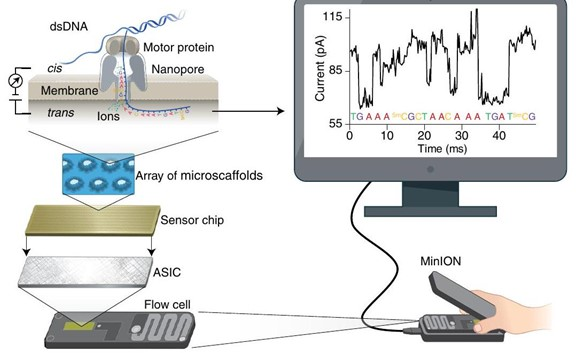
\includegraphics[width=0.8\linewidth]{figure/1mini}
	\caption{MinION nanopore sequencing 原理 \cite{0wang2021nanopore}} \label{MinION}
\end{figure}

图\ref{MinION}展示了MinION纳米孔测序原理.一个MinION Flow细胞包含512个通道,每个通道中有4个纳米孔,总计2,048个纳米孔用于DNA或RNA的测序.纳米孔位于由连接到传感器芯片的微支架阵列支撑的耐电聚合物膜内.每个通道与传感器芯片中的独立电极相连,并由专用集成电路(ASIC)单独控制和测量.由于在膜上施加了恒定电压,离子电流通过纳米孔,膜的反面带正电荷.在马达蛋白质的作用下,首先解开双链DNA(dsDNA)分子(或RNA-DNA杂交双链),然后在电压驱动下,单链DNA或带负电荷的RNA穿过纳米孔.当核苷酸通过纳米孔时,测量特征电流变化,并根据这些变化确定相应的核苷酸类型,每秒约可识别450个碱基(R9.4纳米孔).

原理中涉及到的主要概念和作用:
\begin{enumerate}
	\item 纳米孔:MinION设备包含众多纳米孔,嵌入一层类细胞膜物质(通常为生物膜蛋白).每个纳米孔可检测通过的DNA分子.
	\item 核酸分子穿孔:测序过程中,DNA分子被引导穿过纳米孔.需要对DNA分子进行处理,如加入适配器或线性化.
	\item 电压梯度与电流信号:纳米孔两侧施加电压梯度,使带负电荷的DNA分子受电场驱动穿过纳米孔.DNA分子穿过时,阻碍纳米孔内离子流,改变电流信号.电流信号随DNA中不同碱基(A、T、C和G)的通过而变化.
	\item 信号解码:MinION设备记录纳米孔实时电流信号,用专门算法将信号转换为对应碱基序列.
\end{enumerate}

图\ref{step}展示了DNA通过纳米孔转位的步骤:(i)开放通道;(ii)双链DNA(带有铅接头(蓝色)、结合分子马达(橙色)和发夹接头(红色))被纳米孔捕获;捕获后依次转位的是(iii)铅接头、(iv)模板链(金色)、(v)发夹接头、(vi)互补链(深蓝色)和(vii)拖尾接头(棕色);最后(viii)状态恢复至开放通道.在这个过程中,DNA以特定顺序穿过纳米孔,产生的离子电流信号可以被检测并用于解码DNA序列.

\begin{figure}[htp!]
	\centering
	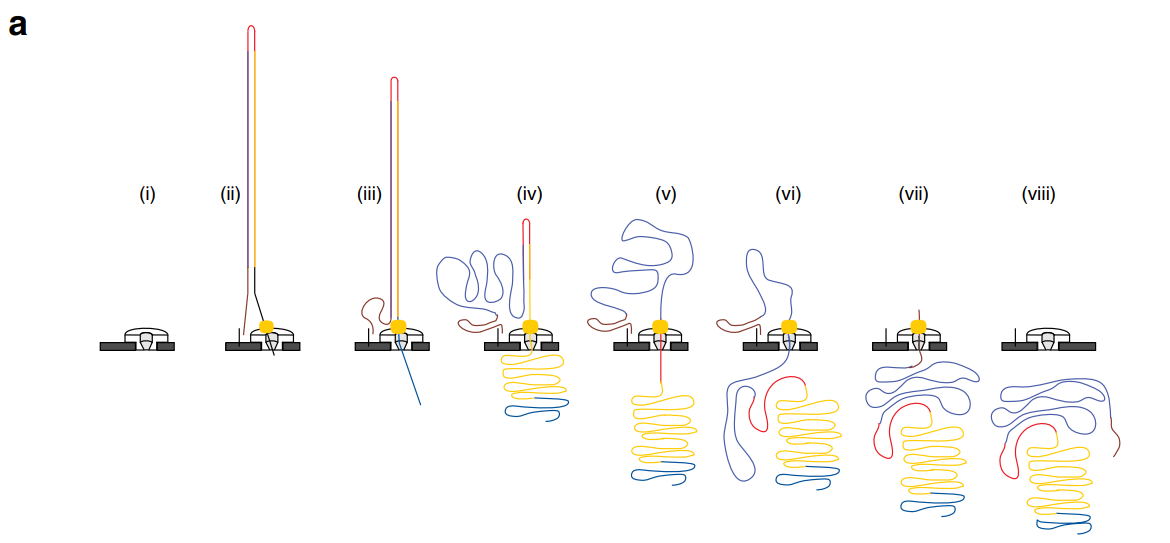
\includegraphics[width=0.8\linewidth]{figure/步骤}
	\caption{MinION nanopore sequencing 步骤 \cite{2jain2016oxford}} \label{step}
\end{figure}

\subsubsection{Basecaller电流信号解码算法}

当DNA分子穿过纳米孔时,不同的碱基(A、T、C和G)会引起电流信号的特异性变化.这些变化取决于每种碱基与纳米孔之间的相互作用,在实际情况中,单个碱基的信号解析很困难,因为测序过程中DNA是以k-mer(一般是3-6个连续碱基)的方式通过纳米孔的.因此,在实际应用中,通常会观察到由连续几个碱基组成的k-mer引起的复合信号.这些信号随着不同k-mer组合的通过而发生变化,可以通过特定的算法进行解码以获取原始的碱基序列.如何精确地将ONT生成的原始电信号翻译为序列信息(即basecalling)也就是科学家们关注的重点,当然也是我这个专业的研究者更关心的,所以还是得专门来讨论一下.


牛津纳米孔公司似乎提供了MinION的云计算服务Metrichor,该方法主要基于隐马尔可夫模型(HMM),但属于闭源软件.为了开发离线的替代方案,一些研究者着手研究开源算法,下面我们将主要讨论在文献\cite{2jain2016oxford}中提到的两种知名的算法Nanocall和DeepNano.

Nanocall\cite{david2017nanocall}是一种基于隐马尔可夫模型HMM的基本呼叫器Basecaller,它在本地执行高效的1D基本呼叫,无需互联网连接,其精度可与牛津纳米孔公司提供的基于Metrichor的1D基本呼叫相媲美.

Nanocall的输入是一组存储在ONT特定的FAST5文件中的分段事件序列.Nanocall分别处理每个输入文件,具体步骤如下.首先,在发现发夹结构时,将模板链和互补链分为单独的事件序列.接下来,它估算孔模型的缩放参数.可选地,Nanocall可以使用期望最大化算法进行多轮训练,以更新缩放参数,并使用标准的Baum-Welch算法\cite{baum1972inequality}更新状态转移参数.最后,Nanocall执行标准的Viterbi解码,以找到隐藏状态的路径,其中状态是纳米孔中的6-mer.对于上述模型中的一些经典算法,应当可以在任何一本随机过程或者生物信息学教材中找到,因此不再赘述.

具体地说,状态转移是从一个状态转移到另一个状态的先验概率.默认的状态转移是基于两个参数计算的:'stay'概率$p_{\text {stay }}$ 和'skip'概率$p_{\text {skip. }}$ 前者,$p_{\text {stay }}$,表示两个连续事件来自同一上下文/状态的概率.这对应于分割错误,即引入了错误的事件分割.后者,$p_{\text {skip }}$,表示两个连续事件来自状态差异超过一个kmer位移的概率.这对应于分割错误或测序错误(即DNA通过孔太快,无法捕捉可检测的事件events),其中一个或多个事件丢失.一个稍微复杂的问题是,通过增加跳过次数,总是有多种从一个状态到另一个状态的方式.例如,ACGTGT可以通过一次或三次跳过后在后面接上GTGTAC.下面对状态转移的计算也考虑到了这一点:
$$
\begin{aligned}
	\tau\left(k_1, k_2\right)= & \delta_{k_1=k_2} \cdot p_{\text {stay }} 
	 +\delta_{\text {suffix }\left(k_1, 5\right)=\operatorname{prefix}\left(k_2, 5\right)} \cdot p_{\text {step }} \cdot \frac{1}{4} \\
	& +\sum_{i=2}^5 \delta_{\text {suffix }\left(k_1, 6-i\right)=\operatorname{prefix}\left(k_2, 6-i\right)} \cdot p_{\text {skip } 1}{ }^{i-1} \cdot \frac{1}{4^i} 
	 +\sum_{i>5} p_{\text {skip } 1}{ }^{i-1} \cdot \frac{1}{4^6} .
\end{aligned}
$$
这里,$\delta$是标准示性函数;$\operatorname{prefix}(k, i) / \operatorname{suffix}(k, i)$是长度为$i$的$k$的前缀/后缀;$p_{\text {step }}:=\left(1-p_{\text {stay }}-p_{\text {skip }}\right)$;而$p_{\text {skip } 1}=p_{\text {skip }} /\left(1+p_{\text {skip }}\right)$对应恰好一个跳过的概率.


在包含隐状态的状态转移矩阵训练之后,Nanocall运行Viterbi解码算法,计算生成观察到的事件序列的最可能的状态序列.之后通过迭代添加在连续状态之间转换所需的最少碱基数来构建最终的碱基序列.例如,连续状态ACTCTC和CTCTCA生成碱基序列ACTCTCA,而不是ACTCTCTCA.特别地,由于这种启发式方法和纳米孔中不变状态的特性,所调用的碱基序列不会包含比kmer大小(6 bp)更长的同源重复序列.然而,仍能检测到长度大于1的重复序列.因此,Nanocall读取在大小为1的重复序列附近可能产生系统性(非随机)错误.

DeepNano\cite{bovza2017deepnano}是一个基于循环神经网络(recurrent neural network)\cite{giles1994dynamic}框架的算法,用于执行基调用,其精度优于基于HMM的方法.在互联网连接有限的情况下进行现场测序时,能够执行本地、离线基地呼叫非常有用.

在图\ref{deepnano}的DeepNano中,给定一组输入向量$\left\{\vec{x}_1, \vec{x}_2, \ldots, \vec{x}_t\right\}$.它的预测是一组输出向量$\left\{\vec{y}_1, \vec{y}_2, \ldots, \vec{y}_t\right\}$. 在这里,我们需要预测DNA序列,因此每个输入向量$\vec{x}_i$包含每个事件(即长度为k的电流信号)的均值、标准差和长度,输出向量$\vec{y}_i$给出了呼叫碱基的概率分布.
在处理每个输入向量$\vec{x}_i$时,循环神经网络计算两个向量:其隐藏状态$\vec{h}_i$和输出向量$\vec{y}_i$.这两者都取决于当前输入向量和之前的隐藏状态:$\vec{h}i=f\left(\vec{h}_{i-1}, \vec{x}_i\right), \vec{y}_i=g\left(\vec{h}_i\right)$.通常,通过使用具有多个隐藏层的神经网络可以提高预测准确性,其中每个层使用来自前一层的隐藏状态.我们使用具有三层或四层的网络.对于三层的计算如下:
$$
\begin{aligned}
	\vec{h}_i^{(1)} & =f_1\left(\vec{h}_{i-1}^{(1)}, \vec{x}_i\right) \\
	\vec{h}_i^{(2)} & =f_2\left(\vec{h}_{i-1}^{(2)}, \vec{h}_i^{(1)}\right) \\
	\vec{h}_i^{(3)} & =f_3\left(\vec{h}_{i-1}^{(3)}, \vec{h}_i^{(2)}\right) \\
	\vec{y}_i & =g\left(\vec{h}_i^{(3)}\right)
\end{aligned}
$$



\begin{figure}[htp!]
	\centering
	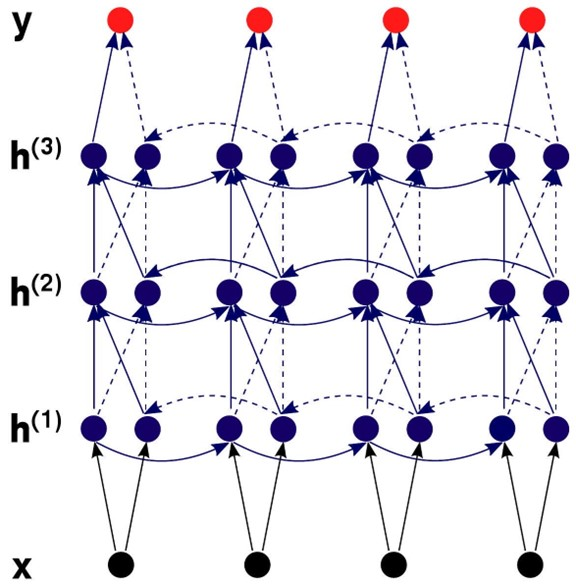
\includegraphics[width=0.8\linewidth]{figure/deepnano}
	\caption{deepnano 循环神经网络模型 \cite{bovza2017deepnano}} \label{deepnano}
\end{figure}



当然,对于上述两种算法循环神经网络和隐马尔可夫模型,实际上我个人认为两者的构造还是非常接近的,因为都存在相应的时序特征需要训练而且都共享训练权重,因此处理DNA序列肯定是有效的.不过如果现在让我设计的话,肯定是要加入预训练和Transformer模型了,时代在不断变化.




\subsubsection{原理总结}

Oxford Nanopore的纳米孔测序技术基于单个DNA分子通过纳米孔的电信号变化来实现.A、C、G、T 四种不同的碱基在电场作用下通过纳米孔时,会产生不同的电信号,这些信号可以被检测和记录下来.这些信号可以被转换成DNA序列,并且可以在实时中进行读取和分析.


\subsection{Oxford Nanopore牛津纳米孔测序技术的优缺点}

\subsubsection{优点}

\begin{enumerate}
	\item 长读长:
	纳米孔测序技术的长读长为DNA或RNA序列比对和匹配带来了优势,有助于获得高质量、更完整的基因组组装.长读长在植物基因组等具有复杂结构和高度重复区域的研究中显著,简化了从头组装过程,改进参考基因组,实现phasing,加快宏基因组物种鉴定.对于RNA,长读长有助于全长转录本表征,及异构体、剪接变体和融合转录本的量化和分析.由电检测提供的读长具有很高上限,依赖核酸转位物理过程,2018年实现了高达2.273兆碱基(Mb)的读长\cite{gong2019ultra}.
	
	\item 高通量:
	ONT测序技术具有较高吞吐量,满足不同项目规模需求.吞吐量提高得益于活跃纳米孔数量增加、DNA/RNA转移速度提升及运行时间延长.早期MinION用户报告每个流动池产量为数百兆碱基,而现吞吐量已增至约10-15千兆碱基(Gb),得益于更快的化学反应(R6纳米孔速度约每秒30个碱基,提高至R9.4纳米孔每秒约450个碱基)及引入Rev D SIC芯片后更长运行时间.后续设备,如PromethION,运行更多流动池,每个流动池纳米孔数量更多\cite{nicholls2019ultra}.
	
	
	\item 实时靶向测序:这是在短时间内获取和分析DNA或RNA序列的有效方法,尤其适用于临床应用.MinION平台因其小型、低成本、简易的文库准备和便携性,使实时分析成为可能\cite{loose2016real}.通过在测序过程中实时捕获和分析DNA链,可以迅速积累目标片段的读取.实时靶向测序技术有助于显著缩短从生物样本收集到数据分析所需的时间,对于现场和临床护理应用具有重要意义.
	
	\item 直接检测碱基修饰:第二代NGS技术无法直接检测原生DNA中的碱基修饰.然而,纳米孔技术可以对原生DNA和RNA的单个核苷酸进行单分子测序,从而检测其中的修饰.比如有研究发现,纳米孔系统能够准确识别五种不同类型的胞嘧啶\cite{wescoe2014nanopores}(包括C、5-甲基胞嘧啶、5-羟甲基胞嘧啶、5-甲酰胞嘧啶和5-羧胞嘧啶),准确率达92\%至98\%.
	
	\item 可直接对RNA表达分析:ONT技术可以直接测序RNA分子,提供更真实的转录本信息,避免了将RNA逆转录成cDNA的步骤.而NGS测序cDNA拷贝的片段较短,导致全长转录本的组装和RNA剪接异构体的准确表征困难.MinION平台可进行全长cDNA读取,例如研究利用MinION成功检测了果蝇中四个基因的RNA剪接变体和异构体,其中一个复杂基因的7000多种异构体的比对同一性高达90\%.这在450个碱基长度的NGS读取中是无法实现的\cite{bolisetty2015determining}.
	
	\item 便携性、简化性与低成本:ONT的便携设备如MinION和Flongle使纳米孔测序技术能在实验室之外的环境中使用,如现场实验和偏远地区.同时,ONT的测序流程无需PCR扩增,避免了PCR偏差和可能的错误.此外,ONT的设备和测序试剂价格相对较低,特别适合小规模实验和个体研究者.
	
\end{enumerate}


\subsubsection{缺点}

\begin{enumerate}
	
	\item 准确性较低:ONT纳米孔测序的一个主要缺点是其较低的测序准确性.与其他测序平台相比,ONT的单次读取准确性通常在85%-90%之间.这可能会影响某些应用,例如单核苷酸多态性(SNP)检测和低丰度变异体的识别.比如图\ref{miss}中显示的结果.
	
	\begin{figure}[htp!]
		\centering
		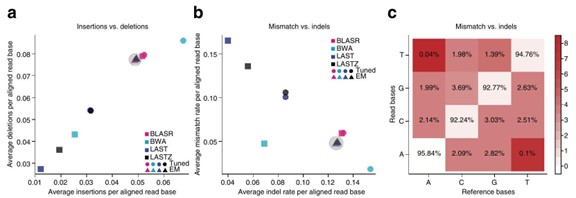
\includegraphics[width=1\linewidth]{figure/miss}
		\caption{MinION测序与参考序列比对结果\cite{2jain2016oxford}} \label{miss}
	\end{figure}
	
	\item 高错误率:ONT测序数据中的错误主要是插入和缺失错误,这可能会对某些应用产生负面影响,例如测序短的重复序列或串联重复序列.比如我们之前提到的Nanocall\cite{david2017nanocall}在大小为1的重复序列附近可能产生的系统性(非随机)错误.
	
	
	\item 数据分析难度大:由于测序产生的大量长读长数据而且还是电信号,数据分析需要较高的计算资源和专业知识,需要使用到比较先进的算法,比如我们之前提到的HMM,RNN,当然之后肯定还需要更先进的深度学习算法.
\end{enumerate}

\subsubsection{与第一、二代测序比较}


\begin{enumerate}
	\item 读长(Read Length):\\
	ONT测序技术可以生成非常长的读长(超过1 Mb),而第一代(例如Sanger测序)和第二代测序技术(例如Illumina)通常具有较短的读长(数百到数千个碱基).
	
	\item 准确性(Accuracy):\\
	ONT测序的准确性相对较低(约85%-90%),而Sanger测序的准确性高达99.99%,Illumina测序的准确性也在99%以上.
	
	\item 通量(Throughput):\\
	ONT测序通量适中,可以根据不同设备满足不同项目规模的需求.Illumina测序具有非常高的通量,适合大规模项目.而Sanger测序的通量相对较低.
	
	\item 实时性(Real-time):\\
	ONT测序技术具有实时分析的能力,可以在测序进行时获取数据.而Sanger测序和Illumina测序在完成整个测序过程后才能获取数据.
	
	\item 样品准备(Sample Preparation):\\
	ONT测序通常不需要PCR扩增,可以避免引入PCR偏差和可能的错误.而Sanger测序和Illumina测序通常需要进行PCR扩增.
	
	\item 成本(Cost):\\
	ONT测序设备和试剂相对较便宜,尤其适合小规模实验和个体研究者.Sanger测序成本适中,但通量较低.Illumina测序在大规模项目中成本效益较高,但对于小规模实验成本可能较高.
	
	\item 便携性(Portability):\\
	ONT的设备(如MinION和Flongle)非常小巧便携,适合现场实验和远程地区.而Sanger测序和Illumina测序设备较大,通常需要固定在实验室中使用.
\end{enumerate}

\subsection{Oxford Nanopore牛津纳米孔测序技术的应用}
    牛津纳米孔测序技术在基础研究、临床应用和现场应用等领域有着广泛的应用.这些应用根据ONT测序的优势,如长读长、原生单分子和便携性等特点,可以进一步细分为多个具体主题.

\begin{figure}[htp!]
	\centering
	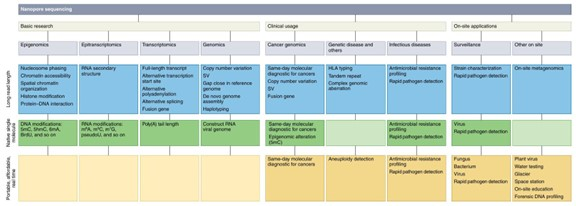
\includegraphics[width=1\linewidth]{figure/ontapp}
	\caption{Oxford Nanopore牛津纳米孔测序技术的应用表 \cite{0wang2021nanopore} } \label{ontapp}
\end{figure}

\subsubsection{填补参考基因组中的空缺}

牛津纳米孔测序技术在基因组组装方面具有显著应用价值,特别是在填补参考基因组中的空缺和识别重复区域方面.人类基因组、线虫参考基因组等已经通过ONT长读长成功地填补了空缺和扩展.在其他模式生物、近缘物种和非模式生物方面也取得了类似的进展,有助于改善这些物种基因组的连续性和完整性.例如,ONT读取已用于关闭人类参考基因组中的12个缺口(每个缺口> 50 kb),测量端粒重复的长度,以及组装人类Y染色体的中心粒区域\cite{jain2018linear}.此外,ONT使得首次实现了人类X染色体的无缺口端粒至端粒组装,包括重建约2.8 Mb的中心粒卫星DNA阵列和关闭所有剩余的29个缺口(总计1.1 Mb)\cite{miga2020telomere}.

\subsubsection{建立新的参考基因组}

牛津纳米孔测序技术在非模式生物初始参考基因组的组装中发挥了重要作用.例如,通过仅使用ONT数据或结合其他技术,成功组装了根腐病菌、澳大利亚最大淡水鱼、普通小丑鱼等物种的基因组.ONT直接RNA测序也被用于构建RNA病毒基因组,无需传统的反转录步骤.在SARS-CoV-2大流行期间,ONT测序通过cDNA和直接RNA测序重建了全长SARS-CoV-2基因组序列,为病毒的生物学、进化和致病性研究提供了重要信息.

\subsubsection{识别大型结构变异(SV)}

牛津纳米孔测序技术在识别大型结构变异方面具有显著优势,特别是在生物医学背景中.例如,它已成功应用于乳腺癌细胞系、急性髓系白血病患者以及具有先天异常的个体.ONT技术还有助于在人类基因组中识别大量结构变异.

\subsubsection{表征全长转录组和复杂转录事件}

ONT cDNA测序技术在表征全长转录组和复杂转录事件方面展现了显著的潜力.与PacBio长读长相比,它在识别基因亚型方面具有相似的性能.虽然在评估基因丰度和检测剪接位点方面存在一定的限制,但准确性和吞吐量的改进正在改善这些分析.ONT技术还用于研究不同生物中的RNA分子的poly(A)尾长以及人类环状RNA的全长亚型.

\subsubsection{检测RNA修饰}

ONT直接RNA测序技术为检测具有关键生物学功能的RNA修饰和RNA编辑提供了新的可能性.通过ONT测序,研究者在不同生物中检测了各种RNA修饰\cite{garalde2018highly},如m6A、m7G和假尿苷.此外,结合人工化学修饰,ONT直接RNA测序可以用于探测RNA的二级结构.同时,通过标记新生RNA并进行ONT直接RNA测序,RNA代谢动态也得到了分析.

\subsubsection{癌症研究治疗}

ONT测序技术已广泛应用于各种癌症类型,以识别复杂的基因组变异.这种技术可以快速检测白血病患者中的突变、染色体易位和断点.同时,ONT测序还能分析具有高重复序列和大基因大小的癌症易感基因.通过直接检测DNA修饰\cite{euskirchen2017same},ONT数据可同时捕获基因组和表观基因组变异.ONT测序技术还可以在短时间内为癌症提供多模式的快速分子诊断.例如,它已成功应用于检测临床样本中的融合基因\cite{jeck2019nanopore}.总之,ONT测序技术在癌症研究中具有显著的应用价值,为更深入地了解癌症相关基因突变和诊断提供了有力工具.